\documentclass[12pt, a4paper]{article}


\usepackage{xeCJK}

\usepackage{amsmath, amssymb} 
\usepackage{graphicx}       
\usepackage{geometry}
\usepackage{enumitem}
\usepackage{setspace}
\usepackage{tikz}
\usetikzlibrary{shapes.geometric, arrows.meta, positioning}
\geometry{top=2.5cm, bottom=2.5cm, left=2.5cm, right=2.5cm}

\title{PA1 Report}
\author{}
\date{}

\begin{document}

\maketitle
\vspace{-2.0cm} % 減少標題下方的空白

\section*{Problem 1:}

\subsection*{Question 1:}

In -O0, What is the memory byte stride (the address distance in bytes between \texttt{in[i]} and \texttt{in[i+1]})?

\vspace{0.3cm}
\noindent\fbox{\textbf{Answer:}}\\
Since in -O0 optimization, the 15th line of the RISC-V assembly code is \texttt{slli a5,a5,3}, which multiplies the index value in register \texttt{a5} by 8 (since $2^3 = 8$). This offset is then added to the base address of the array \texttt{in} (stored in \texttt{a4}) so that \texttt{a5} becomes the address of \texttt{in[i]}. This means the address distance between \texttt{in[i]} and \texttt{in[i+1]} is 8 bytes.

\noindent\hrulefill

\vspace{0.3cm}
\noindent
Why does this stride differ from \texttt{sizeof(char) + sizeof(int)}? Draw a memory layout diagram of a single struct Record showing byte offsets
and padding. 

\vspace{0.3cm}
\noindent\fbox{\textbf{Answer:}}\\
The stride (8 bytes) differs from \texttt{sizeof(char) + sizeof(int)} ($1 + 4 = 5$ bytes) due to memory alignment and data structure padding. 

In C, compilers automatically align data in memory to optimize CPU memory access. An \texttt{int} typically requires a 4-byte alignment (its memory address must be a multiple of 4). If a struct contains a \texttt{char} (1 byte) and an \texttt{int} (4 bytes), the compiler will insert 3 bytes of "padding" to ensure the \texttt{int} is properly aligned. This makes the total size of the struct $1 + 3 \text{ (padding)} + 4 = 8$ bytes. This is why the memory stride between elements is 8 bytes instead of 5 bytes.

\begin{table}[h]
\centering
\renewcommand{\arraystretch}{1.5}
\begin{tabular}{|c|c|c|c|c|c|c|c|}
\hline
\multicolumn{8}{|c|}{a single struct Record (8 bytes total)} \\
\hline
\textbf{+0} & \textbf{+1} & \textbf{+2} & \textbf{+3} & \textbf{+4} & \textbf{+5} & \textbf{+6} & \textbf{+7} \\
\hline
\texttt{char} & \multicolumn{3}{c|}{Padding (3 bytes)} & \multicolumn{4}{c|}{\texttt{int} (4 bytes)} \\
\hline
\end{tabular}
\end{table}

\noindent\hrulefill

\vspace{0.3cm}
\noindent
In -O0, why does the loop body contain frequent lw and sw instructions for local variables?

\vspace{0.3cm}
\noindent\fbox{\textbf{Answer:}}\\
Under -O0 (no optimization), the compiler prioritizes compilation speed and debugging ability over runtime performance. It does not perform register allocation to keep local variables in CPU registers across different statements. Instead, every local variable is assigned a fixed location in memory (on the stack). 

Whenever a variable is read, it must be fetched from memory into a register using a load word (\texttt{lw}) instruction. Whenever a variable is modified, its new value must be immediately written back to its stack memory location using a store word (\texttt{sw}) instruction. This strict memory mapping ensures that the memory always contains the most up-to-date values of all variables.

\noindent\hrulefill

\vspace{0.3cm}
\noindent
How does -O1 optimize register allocation to eliminate the stack frame and transform array indexing into pointer bumping (addi)?

\vspace{0.3cm}
\noindent\fbox{\textbf{Answer:}}\\
Based on the \texttt{-O1} assembly, the compiler applies these two optimizations clearly:
\begin{itemize}[leftmargin=*]
    \item \textbf{Eliminating the Stack Frame (Register Allocation):} There is no \texttt{addi sp, sp, -XX} at the beginning of the function. The compiler allocates all local variables and pointers directly to CPU registers (e.g., the accumulator is kept purely in \texttt{a4} with \texttt{li a4,0} and \texttt{add a4,a4,a2}). Since no variables are "spilled" to memory, no stack frame is needed.
    \item \textbf{Pointer Bumping:} Instead of maintaining a loop index $i$ and computing the address on every iteration (\texttt{in + i * 8}), the compiler initializes \texttt{a0} to point directly to \texttt{in[0].val} (\texttt{addi a0, a0, 4}). At the end of each loop iteration (label \texttt{.L4}), it simply advances the pointer by the struct's stride of 8 bytes using \texttt{addi a0, a0, 8}. It also bumps the output pointer by 4 bytes (\texttt{addi a5, a5, 4}). This replaces costly multiplication/shift operations inside the loop with simple, fast addition.
\end{itemize}

\vspace{5pt}
\hrule height 0.5pt
\vspace{2pt}
\hrule height 0.5pt
\vspace{5pt}

\subsection*{Question 2:}

\vspace{0.3cm}
In -O1, identify the instruction sequence for acc / 4. Trace through an example
with a negative dividend (e.g., −5) to explain why an arithmetic right shift alone
(srai) produces an incorrect result for C signed integer division.

\vspace{0.3cm}
\noindent\fbox{\textbf{Answer:}}\\
In the -O1 assembly, the instruction sequence for \texttt{acc / 4} (found under \texttt{.L8}) is:
\begin{verbatim}
srai a2, a4, 31
andi a2, a2, 3
add  a2, a2, a4
srai a2, a2, 2
\end{verbatim}

In C, integer division is defined to truncate towards zero. If we simply use an arithmetic right shift (\texttt{srai a2, a4, 2}) to divide by 4 ($2^2$), it rounds towards negative infinity. This works fine for positive numbers but produces the wrong result for negative numbers.

\noindent
\textbf{Example Trace with -5 (\texttt{a4 = -5})}:
\begin{enumerate}[leftmargin=*]
    \item In C, \texttt{-5 / 4} should equal \texttt{-1} (truncating towards zero).
    \item Why \texttt{srai} alone fails: \texttt{-5} is represented in two's complement as \texttt{...1111 1011}. If we just shift it right by 2 (\texttt{-5 >> 2}), we get \texttt{...1111 1110}, which is \textbf{\texttt{-2}}. This is incorrect!
\end{enumerate}

\noindent\hrulefill

\vspace{0.3cm}
\noindent
In -O1, how is acc / 10 implemented without a hardware division instruction?
Identify the constant used and explain how high-word multiplication (mulh) achieves
division.

\vspace{0.3cm}
\noindent\fbox{\textbf{Answer:}}\\
To compute \texttt{acc / 10} without a costly hardware division instruction, the compiler uses a technique called division by invariant multiplication.

\noindent
\textbf{1. Identifying the Constant:}\\
The assembly initializes a constant using:
\begin{verbatim}
li   t1, 1717985280
addi t1, t1, 1639
\end{verbatim}
\begin{spacing}{1.4}
The sum is $1717985280 + 1639 = 1717986919$. Specifically, it is the ceiling of $\dfrac{2^{34}}{10}$ ($\lceil 1717986918.4 \rceil = 1717986919$). The tiny $+0.6$ offset acts as a precision correction.
\end{spacing}

\noindent
\textbf{2. How High-Word Multiplication (\texttt{mulh}) Achieves Division:}\\
The sequence of instructions is:
\begin{verbatim}
mulh a2, a4, t1
srai a2, a2, 2
srai t3, a4, 31
sub  a2, a2, t3
\end{verbatim}
\begin{spacing}{1.4}
\begin{itemize}[leftmargin=*]
    \item \texttt{mulh a2, a4, t1}: This multiplies the accumulator (\texttt{a4}) by the 32-bit constant (\texttt{t1}) to produce a 64-bit product, but it only stores the \textbf{upper 32 bits} into \texttt{a2}. Taking the upper 32 bits of a 64-bit product is mathematically equivalent to dividing the product by $2^{32}$. Thus, this step computes $\dfrac{\text{acc} \times (\frac{2^{34}}{10} + 0.6)}{2^{32}}$. Because the precision correction term $\dfrac{\text{acc} \times 0.6}{2^{32}}$ is vanishingly small (always $< 1$ for 32-bit integers), it is safely truncated, leaving us with approximately $\dfrac{\text{acc} \times 2^{34}/10}{2^{32}} = \dfrac{\text{acc} \times 2^2}{10} = \dfrac{\text{acc} \times 4}{10}$.
    \item \texttt{srai a2, a2, 2}: This arithmetic right shift by 2 effectively divides the previous result by $2^2$ (which is 4). Doing so yields exactly $\dfrac{\text{acc}}{10}$.
    \item \textbf{Sign Correction (\texttt{srai} and \texttt{sub}):} C requires integer division to truncate towards zero. For negative dividends, the right shifts will round towards negative infinity. \texttt{srai t3, a4, 31} copies the sign bit of the original accumulator (-1 if negative, 0 if positive). \texttt{sub a2, a2, t3} subtracts this sign mask. If the original number was negative, it subtracts -1 (effectively adding 1), correcting the rounding direction so it accurately truncates towards zero.
\end{itemize}
\end{spacing}

\noindent\hrulefill

\vspace{0.3cm}
\noindent
Recompile under -O2 with -march=rv32i -mabi=ilp32. How does the implementation of acc / 10 change?

\vspace{0.3cm}
\noindent\fbox{\textbf{Answer:}}\\
Under -O2 with \texttt{-march=rv32i}, the implementation of \texttt{acc / 10} completely abandons the "magic number division" trick and instead falls back to a software function call. The assembly changes to:
\begin{verbatim}
li   a1, 10
mv   a0, s1
call __divsi3
\end{verbatim}

\noindent\hrulefill

\vspace{0.3cm}
\noindent
According to the RISC-V calling convention, why does this function now need to set up a stack frame and save
ra and s-registers?

\vspace{0.3cm}
\noindent\fbox{\textbf{Answer:}}\\
Because the function must now call \texttt{\_\_divsi3}, it is no longer a \textbf{leaf function} (a function that doesn't call other functions). According to the RISC-V calling convention, this fundamentally changes how registers must be managed:

\begin{spacing}{1.4}
\begin{itemize}[leftmargin=*]
    \item \textbf{Saving the Return Address (\texttt{ra}):} When \texttt{process\_records} calls \texttt{\_\_divsi3}, the \texttt{call} instruction overwrites the \texttt{ra} register with the return address. If the original \texttt{ra} is not saved to the stack, the function will forget how to return to whoever originally called it.
    \item \textbf{Saving Callee-Saved Registers (\texttt{s0}-\texttt{s5}):} Because \texttt{\_\_divsi3} is an external function call, it is allowed to freely overwrite caller-saved temporary registers (\texttt{t0}-\texttt{t6}, \texttt{a0}-\texttt{a7}). To ensure that important loop variables (like pointers, loop bounds, and the accumulator) survive across the division call, the compiler must allocate them to \textbf{callee-saved registers} (\texttt{s0}-\texttt{s5}). However, the convention dictates that if a function modifies any \texttt{s}-registers, it must first save their original values to the stack and restore them before returning, so it doesn't corrupt its caller's data.
    \item \textbf{Setting up the Stack Frame:} To have a safe place in memory to store the \texttt{ra} and these six \texttt{s}-registers, the function must allocate 32 bytes of space on the stack (\texttt{addi sp, sp, -32}) at the prologue, effectively creating a stack frame.
\end{itemize}
\end{spacing}

\vspace{5pt}
\hrule height 0.5pt
\vspace{2pt}
\hrule height 0.5pt
\vspace{5pt}

\subsection*{Question 3:}

\vspace{0.3cm}
Compare the loop structures between -O2 and -O3. How many distinct loop blocks exist in each version? Draw simplified control-flow graphs (CFGs) for both levels.

\vspace{0.3cm}
\noindent\fbox{\textbf{Answer:}}\\
\textbf{Number of Distinct Loop Blocks:}
\begin{spacing}{1.4}
\begin{itemize}[leftmargin=*]
    \item \textbf{-O3 (3 distinct loop blocks):} The compiler evaluates the \texttt{scale\_mode} condition exactly once outside the loops. It branches to three entirely separate, specialized loop bodies (\texttt{.L5}, \texttt{.L8}, \texttt{.L7}). Inside these loops, there are zero \texttt{if (scale\_mode == ...)} checks.
    \item \textbf{-O2 (2 distinct loop blocks, 1 shared):} The compiler separates the \texttt{scale\_mode == 1} loop into its own independent block (\texttt{.L5} $\leftrightarrow$ \texttt{.L13}). However, for \texttt{scale\_mode == 2} and the \texttt{default} mode, it shares the common data-loading and accumulator-adding basic block (\texttt{.L9}). Because this block is shared, the compiler must insert a conditional branch (\texttt{bne a3, a7, .L12}) \textit{inside} the loop to determine whether to jump back to the default math block (\texttt{.L12}) or the \texttt{scale\_mode == 2} math block (\texttt{.L6}).
\end{itemize}
\end{spacing}

\noindent
\textbf{Simplified Control-Flow Graphs (CFGs):}

\begin{center}
\textbf{-O3 CFG (Full Loop Unswitching)}\\[0.2cm]
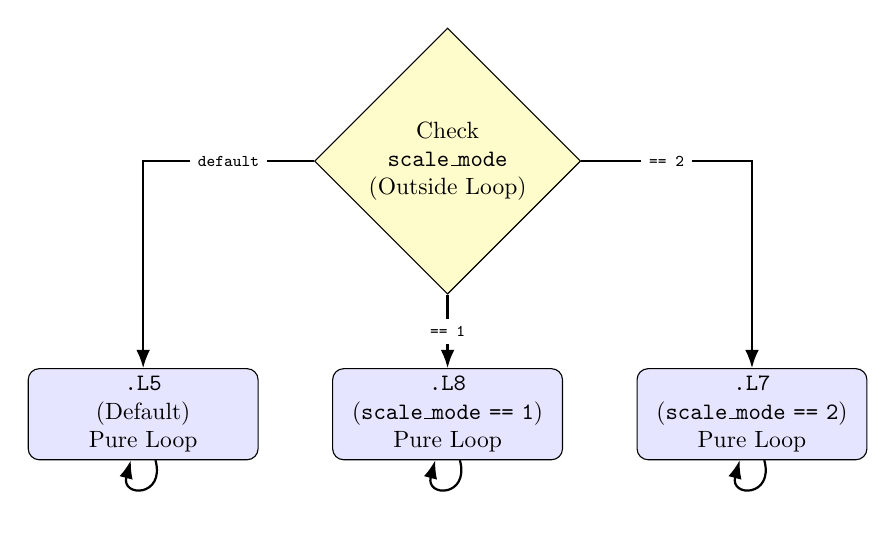
\begin{tikzpicture}[scale=0.85, transform shape,
    node distance=1.1cm and 1.1cm,
    block/.style={rectangle, draw, fill=blue!10, text width=3.2cm, text centered, rounded corners, minimum height=1.2cm},
    decision/.style={diamond, draw, fill=yellow!20, text width=2.8cm, text badly centered, inner sep=0pt},
    line/.style={draw, -Latex, thick}
]
% Nodes
\node [decision] (check) {Check \texttt{scale\_mode}\\(Outside Loop)};
\node [block, below=1.1cm of check] (l8) {\texttt{.L8} \\(\texttt{scale\_mode == 1})\\Pure Loop};
\node [block, left=1.1cm of l8] (l5) {\texttt{.L5} \\(Default)\\Pure Loop};
\node [block, right=1.1cm of l8] (l7) {\texttt{.L7} \\(\texttt{scale\_mode == 2})\\Pure Loop};

% Edges
\path [line] (check) -| node[fill=white, font=\scriptsize, pos=0.25] {\texttt{default}} (l5);
\path [line] (check) -- node[fill=white, font=\scriptsize] {\texttt{== 1}} (l8);
\path [line] (check) -| node[fill=white, font=\scriptsize, pos=0.25] {\texttt{== 2}} (l7);

\path [line] (l5) edge[loop below, looseness=4] node{} (l5);
\path [line] (l8) edge[loop below, looseness=4] node{} (l8);
\path [line] (l7) edge[loop below, looseness=4] node{} (l7);
\end{tikzpicture}

\vspace{0.3cm}
\begin{minipage}{\textwidth}
\centering
\textbf{-O2 CFG (Partial Sharing)}\\[0.2cm]
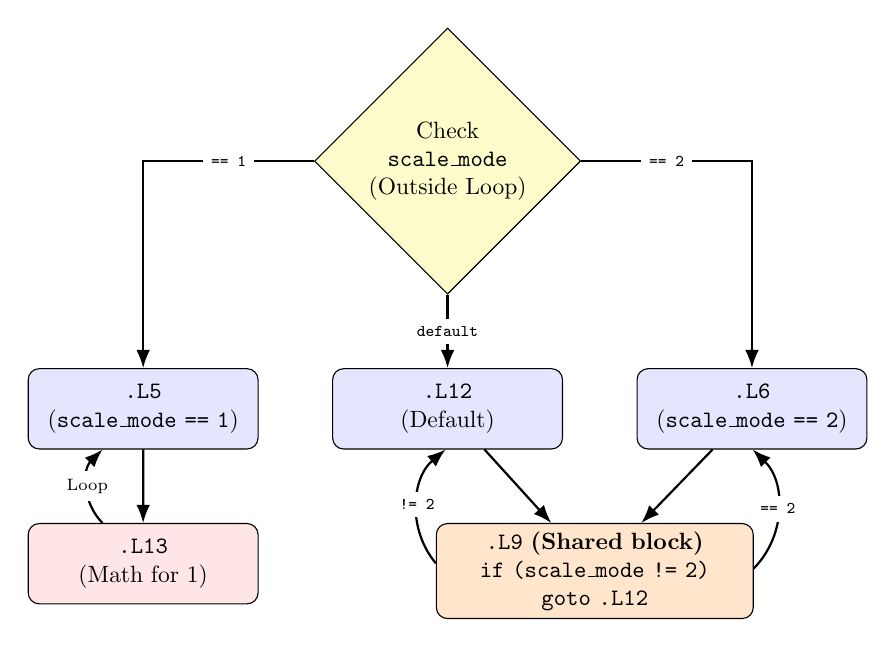
\begin{tikzpicture}[scale=0.85, transform shape,
    node distance=1.1cm and 1.1cm,
    block/.style={rectangle, draw, fill=blue!10, text width=3.2cm, text centered, rounded corners, minimum height=1.2cm},
    decision/.style={diamond, draw, fill=yellow!20, text width=2.8cm, text badly centered, inner sep=0pt},
    line/.style={draw, -Latex, thick}
]
% Nodes
\node [decision] (check) {Check \texttt{scale\_mode}\\(Outside Loop)};
\node [block, below=1.1cm of check] (l12) {\texttt{.L12} \\(Default)};
\node [block, left=1.1cm of l12] (l5) {\texttt{.L5} \\(\texttt{scale\_mode == 1})};
\node [block, right=1.1cm of l12] (l6) {\texttt{.L6} \\(\texttt{scale\_mode == 2})};

\node [block, fill=red!10, below=1.1cm of l5] (l13) {\texttt{.L13} \\(Math for 1)};
\node [block, fill=orange!20, below=1.1cm of l12, xshift=2.2cm, text width=4.5cm] (l9) {\textbf{\texttt{.L9} (Shared block)} \\ \texttt{if (scale\_mode != 2)} \\ \texttt{goto .L12}};

% Edges
\path [line] (check) -| node[fill=white, font=\scriptsize, pos=0.25] {\texttt{== 1}} (l5);
\path [line] (check) -- node[fill=white, font=\scriptsize] {\texttt{default}} (l12);
\path [line] (check) -| node[fill=white, font=\scriptsize, pos=0.25] {\texttt{== 2}} (l6);

\path [line] (l5) -- (l13);
\path [line] (l13) edge[bend left=45] node[fill=white, font=\scriptsize] {Loop} (l5);

\path [line] (l12) -- (l9);
\path [line] (l6) -- (l9);

\path [line] (l9) edge[bend left=45] node[fill=white, font=\scriptsize] {\texttt{!= 2}} (l12);
\path [line] (l9) edge[bend right=45] node[fill=white, font=\scriptsize] {\texttt{== 2}} (l6);
\end{tikzpicture}
\end{minipage}
\end{center}

\noindent\hrulefill

\vspace{0.3cm}
\noindent
Where are the conditional branch checks on \texttt{scale\_mode} placed in -O2 versus -O3? Explain why hoisting invariant checks outside the loop reduces total dynamic instruction execution count per iteration.

\vspace{0.3cm}
\noindent\fbox{\textbf{Answer:}}
\vspace{-0.2cm}
\begin{spacing}{1.4}
\begin{itemize}[leftmargin=*]
    \item \textbf{Placement in -O3:} The conditional checks for \texttt{scale\_mode} are evaluated strictly outside the loops. Once \texttt{scale\_mode} is determined, the program jumps into a specialized, pure loop body (\texttt{.L5}, \texttt{.L8}, or \texttt{.L7}) that contains zero \texttt{scale\_mode} checks.
    \item \textbf{Placement in -O2:} While an initial check is done outside the loop, the compiler shares a basic block (\texttt{.L9}) for two of the loops. Because of this sharing, it must place an additional conditional branch (\texttt{bne a3, a7, .L12}) inside the loop to check \texttt{scale\_mode} on every single iteration.
\end{itemize}

\noindent
\textbf{Why Hoisting Reduces Dynamic Instruction Count:} \\
A loop-invariant condition (like \texttt{scale\_mode}) does not change its value during the loop's execution. If the check is placed inside the loop, the CPU is forced to execute the comparison and branch instructions $N$ times (where $N$ is the number of array elements). By hoisting the check outside the loop (Loop Unswitching), the CPU only evaluates the condition exactly once. This eliminates $N$ redundant conditional branch instructions, significantly reducing the total dynamic instruction count and preventing potential pipeline flushes from branch mispredictions.
\end{spacing}

\end{document}